\chapter{Zadatak 4 --- provjera rješenja i zatvoreni krug}
\label{ch:z4-provjera}

\section{Što se ovdje radi}

Dobiveni $K$ treba \emph{provjeriti}, a ne samo prijaviti. Provjera ide u tri
razine: svojstvene vrijednosti obaju modova zatvorenog kruga, Ljapunovljeve
nejednakosti s dobivenom $P$, i simulacija.

\begin{predznanje}
\begin{itemize}[nosep,leftmargin=*]
  \item $P$ i $K$ iz \eqref{eq:z4-rjesenje}.
  \item Uvjet kvadratne stabilnosti \eqref{eq:z4-kvadratna}.
  \item Eksponencijalna ocjena s Predavanja 7 --- \S\ref{sec:z4-ljapunov}.
\end{itemize}
\end{predznanje}

\section{Prva razina: svojstvene vrijednosti zatvorenog kruga}
\label{sec:z4-eig-zk}

\begin{korak}[Matrice zatvorenog kruga]
Uz $B = \begin{bsmallmatrix} 1 \\ 0 \end{bsmallmatrix}$ i
$K = [-3{,}424629,\ -0{,}104650]$ je
$BK = \begin{bsmallmatrix} -3{,}424629 & -0{,}104650 \\ 0 & 0 \end{bsmallmatrix}$
--- regulator mijenja \emph{samo prvi redak}, jer $B$ ima nulu u drugom.
\begin{align}
A_{\mathrm{parno}} + BK &= \begin{bmatrix} -4{,}424629 & -0{,}628249 \\ 4{,}712389 & -1{,}000000 \end{bmatrix}, \\
A_{\mathrm{neparno}} + BK &= \begin{bmatrix} -4{,}424629 & -4{,}817039 \\ 0{,}523599 & -1{,}000000 \end{bmatrix},
\end{align}
sa svojstvenim vrijednostima
\begin{align}
\lambda(A_{\mathrm{parno}} + BK) &= -2{,}712315 \pm 0{,}168908\,j, \\
\lambda(A_{\mathrm{neparno}} + BK) &= \{-3{,}352491,\ -2{,}072138\} .
\end{align}
Oba su moda zatvorenog kruga Hurwitzova, i to znatno ,,dublje`` nego prije: realni
dijelovi su oko $-2$ do $-3{,}4$ umjesto $-1$. Neparni mod je čak izgubio
oscilatorno ponašanje --- polovi su realni.
\end{korak}

\begin{zamka}[Zamka: to još uvijek nije dokaz]
Hurwitzovost obaju modova zatvorenog kruga je \textbf{nužan, ali ne i dovoljan}
uvjet --- podzadatak b) je pokazao točno to, na otvorenom krugu. Dokaz daje tek
zajednička Ljapunovljeva funkcija. Ako na obrani staneš na svojstvenim
vrijednostima, izložio si se pitanju ,,pa zar niste malo prije pokazali da to ne
znači ništa?``
\end{zamka}

\section{Druga razina: Ljapunovljeve nejednakosti}
\label{sec:z4-provjera-lyap}

\begin{korak}[Prava provjera]
Uvrsti dobivenu $P$ u \eqref{eq:z4-kvadratna} i izračunaj najveću svojstvenu
vrijednost obiju matrica:
\begin{align}
\lambda_{\max}\bigl((A_{\mathrm{parno}} + BK)\trans P + P(A_{\mathrm{parno}} + BK)\bigr) &= -0{,}910478 < 0, \\
\lambda_{\max}\bigl((A_{\mathrm{neparno}} + BK)\trans P + P(A_{\mathrm{neparno}} + BK)\bigr) &= -0{,}329090 < 0 .
\end{align}
Obje su strogo negativne, pa je \eqref{eq:z4-kvadratna} zadovoljen i
$V(x) = x\trans P x$ strogo pada duž trajektorija \emph{oba} moda. To je dokaz
eksponencijalne stabilnosti zatvorenog kruga --- za bilo koji zakon prespajanja.

Uočimo i da je uvjet ,,tješnji`` za neparni mod ($-0{,}329$ nasuprot $-0{,}910$):
on je taj koji ograničava zajamčenu stopu konvergencije.
\end{korak}

\begin{korak}[Odakle stopa $\alpha$]
Iz $\dot{V} \leq -2\alpha V$ slijedi $V(x(t)) \leq V(x(0))e^{-2\alpha t}$, a
odatle ocjena norme s predfaktorom $\sqrt{\operatorname{cond}(P)}$ (Predavanje 7,
slajd 6/37). Brojevi:
\begin{equation}
\alpha = 0{,}288374\ \mathrm{s}^{-1},
\qquad
\sqrt{\operatorname{cond} P} = \sqrt{\frac{1{,}000000}{0{,}563600}} = 1{,}332031,
\end{equation}
\begin{equation}
\norm{x(t)} \leq 1{,}3320\, e^{-0{,}2884\,t}\,\norm{x(0)} .
\label{eq:z4-ocjena}
\end{equation}
Predfaktor veći od jedan znači da norma smije \emph{privremeno porasti} prije
nego počne padati --- i doista, na slici zatvorenog kruga $x_2$ najprije naraste
do $0{,}64$ pa tek onda pada. Ljapunovljeva funkcija $V$ pada monotono; norma
$\norm{x}$ ne mora, jer elipse $V = c$ nisu kružnice.
\end{korak}

\begin{korak}[Koliko je ocjena konzervativna]
Spektralni radijus monodromijske matrice zatvorenog kruga iznosi
\begin{equation}
\rho(\Phi_{\mathrm{cikl}}^{\mathrm{zk}}) = 0{,}069720 \ll 1 .
\end{equation}
To odgovara stopi $-\tfrac12\ln 0{,}06972 \approx 1{,}33\ \mathrm{s}^{-1}$, dakle
oko četiri i pol puta bržoj kontrakciji od zajamčenih $0{,}2884$. Razlog nije
greška: ocjena \eqref{eq:z4-ocjena} vrijedi za \emph{proizvoljno} prespajanje ---
uključujući i najgore moguće --- dok je $\rho$ izračunat za zadano periodičko
prespajanje. Zajamčena ocjena mora pokriti i slučajeve gori od stvarnog.
\end{korak}

\begin{lstlisting}[style=outputstyle]
lambda_max(A_cl,parno'P + P A_cl,parno)     = -0.910478  < 0
lambda_max(A_cl,neparno'P + P A_cl,neparno) = -0.329090  < 0
rho(Phi_cl,cycle) = 0.069720  << 1
alpha = 0.288374 1/s  ->  V(x(t)) <= V(x(0))*exp(-2*alpha*t)
sqrt(cond(P)) = 1.332031  ->  ||x(t)|| <= 1.3320*exp(-0.2884*t)*||x(0)||
\end{lstlisting}

\section{Treća razina: simulacija}
\label{sec:z4-simulacija-zk}

Zatvoreni krug simulira se istim postupkom kao u
Poglavlju~\ref{ch:z4-simulacija}, uz zamjenu $A_i \to A_i + BK$.

\begin{figure}[H]
\centering
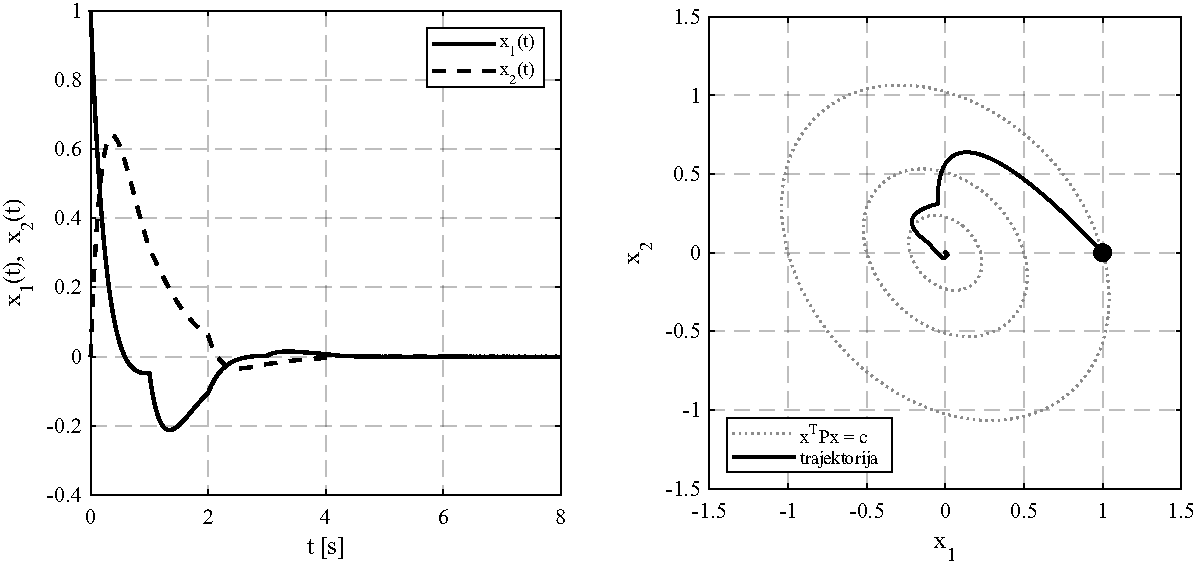
\includegraphics[width=0.95\linewidth]{../figures/fig4_2_closed_loop_stabilization.pdf}
\caption{Zatvoreni krug uz $x(0) = [1,\,0]\trans$: vremenski odziv (lijevo) i
trajektorija u prostoru stanja s nivo-elipsama $x\trans P x = c$ (desno).
Slika 5.2 seminara v1.2.}
\label{fig:z4-zatvoreni}
\end{figure}

\begin{longtable}{@{}p{0.30\linewidth} p{0.66\linewidth}@{}}
\toprule
\textbf{Element} & \textbf{Što je i što pokazuje} \\
\midrule
\endhead
Lijevi graf & Vremenski odziv, $t$ od $0$ do $8$ s (dulje nije potrebno --- sve je
već palo na nulu). \\[5pt]
$x_1(t)$, puna krivulja & Kreće od $1$, strmo pada, prebacuje na $-0{,}21$ oko
$t = 1{,}3$ s, pa se smiruje. \\[5pt]
$x_2(t)$, crtkana krivulja & Kreće od $0$, \emph{raste} do $0{,}64$ oko
$t = 0{,}4$ s, pa pada. Ovo je onaj privremeni porast koji predfaktor
$1{,}3320$ u \eqref{eq:z4-ocjena} dopušta. \\[5pt]
Desni graf, točkaste elipse & Nivo-krivulje Ljapunovljeve funkcije
$x\trans P x = c$. Nagnute su i izdužene jer $P$ nije višekratnik jedinične
matrice. \\[5pt]
Desni graf, puna krivulja & Trajektorija. Kreće iz $(1,\,0)$ i spiralno se
namotava prema ishodištu. \\[5pt]
Odnos krivulje i elipsa & Trajektorija elipse siječe \textbf{uvijek prema
unutra}, nikad prema van. To je slika uvjeta $\dot{V} < 0$ i vizualni dokaz da
je $V$ prava Ljapunovljeva funkcija za oba moda. \\
\bottomrule
\end{longtable}

Brojčano: $\norm{x(5)} = 1{,}52 \cdot 10^{-3}$ i
$\norm{x(20)} = 4{,}72 \cdot 10^{-12}$. Usporedbe radi, u otvorenom krugu je
$\norm{x(20)} = 7{,}19$.

\begin{lstlisting}[style=outputstyle]
--- Simulacija (x(0) = [1; 0], ode45, RelTol 1e-9) ---
otvoreni krug : ||x(20)|| = 7.1868e+00
zatvoreni krug: ||x(5)||  = 1.5176e-03,  ||x(20)|| = 4.7232e-12
\end{lstlisting}

\begin{ploca}[Kako nacrtati sliku zatvorenog kruga]
\begin{enumerate}[leftmargin=*]
  \item Osi $x_1$, $x_2$, raspon $-1{,}5$ do $1{,}5$.
  \item Nacrtaj dvije-tri koncentrične \emph{nagnute} elipse oko ishodišta ---
        to su nivo-krivulje $x\trans P x = c$. Točkasto, tanko.
  \item Označi početnu točku $(1,\,0)$ punom točkom, na rubu najveće elipse.
  \item Iz nje crtaj krivulju koja se namotava prema ishodištu, i to tako da
        \emph{siječe} svaku elipsu prema unutra.
  \item Uz sjecište nacrtaj mali kut između trajektorije i tangente elipse i
        napiši $\dot{V} < 0$.
  \item Reci naglas: ,,trajektorija nivo-elipse siječe uvijek prema unutrašnjosti,
        što je slika uvjeta da Ljapunovljeva funkcija strogo pada; nivo-skup je
        invarijantan``.
\end{enumerate}
\end{ploca}

\begin{izgovor}
,,Dobiveni regulator provjerio sam na tri razine.

Prvo, svojstvene vrijednosti obaju modova zatvorenog kruga: minus dva zarez
sedam jedan plus minus je nula zarez jedan sedam za parni, i dvije realne, minus
tri zarez tri pet i minus dva zarez nula sedam, za neparni. Oba su Hurwitzova ---
ali to je nužan, ne dovoljan uvjet, kako sam pokazao pod b).

Drugo, i to je pravi dokaz: uvrstio sam dobivenu pe u Ljapunovljeve nejednakosti.
Najveće svojstvene vrijednosti su minus nula zarez devet jedan i minus nula zarez
tri tri, obje strogo negativne. Dakle iks transponirano pe iks strogo pada duž
trajektorija oba moda, pa je zatvoreni krug eksponencijalno stabilan za bilo koji
zakon prespajanja.

Iz toga slijedi i ocjena: norma stanja manja ili jednaka jedan zarez tri tri dva
puta e na minus nula zarez dva osam osam te, puta norma početnog stanja.
Predfaktor veći od jedan dopušta privremeni porast norme, što se i vidi --- iks
dva najprije naraste do nula zarez šest četiri.

Treće, simulacija: norma pada s jedan na četiri puta deset na minus dvanaest u
dvadeset sekundi. Na faznom portretu trajektorija siječe nivo-elipse funkcije ve
uvijek prema unutra.

Napomenuo bih da je zajamčena stopa nula zarez dva osam osam konzervativna:
spektralni radijus monodromijske matrice zatvorenog kruga je nula zarez nula
sedam, dakle stvarna kontrakcija je oko četiri puta brža. Razlika postoji jer
ocjena vrijedi za proizvoljno prespajanje, a spektralni radijus za zadano
periodičko.``
\end{izgovor}
